
\documentclass[10pt]{standalone}
\input{../tikzpic_packages.tex}
\begin{document}
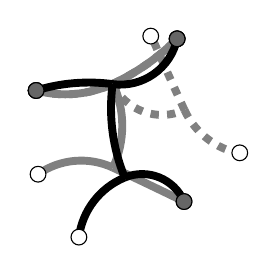
\begin{tikzpicture}
\tikzset{
    part/.style={line width = 1mm, color=gray},
    partD/.style={line width = 1mm, color=gray, dashed},
    partF/.style={line width = 1mm, color=black},
    foot/.style={fill=white},
    footfixed/.style={fill=\col},
    grid line/.style={white},
    start line/.style={help lines}}
\def\rfoot{.1}


\def\col{black!20}
\def\alpi{40.000000}
\def\beti{20.000000}
\def\gam{-50.000000}
\def\alpii{60.000000}
\def\betii{1.000000}
\def\gamh{-25.000000}

\def\eps{90.000000}
\def\ci{75.000000}
\def\cii{135.000000}
\def\ciii{305.000000}
\def\civ{244.000000}

\def\ri{1.432394}
\def\rii{2.864789}
\def\rg{-1.260507}
\def\riii{0.954930}
\def\riv{57.295780}

\path (0.000000, 2.000000)coordinate(F1);

\draw[part] (F1)arc(180+\ci:180+\ci+\alpi:\ri)coordinate(OM);
\draw[part] (OM)arc(180+\ci+\alpi:180+\ci+\alpi+\beti:\rii)coordinate(F2);
\draw[part] (OM)arc(90+\ci+\alpi:90+\ci+\alpi+\gam:\rg)coordinate(UM);
\draw[part] (UM)arc(\gam+\ci+\alpi:\gam+\ci+\alpi+\alpii:\riii)coordinate(F3);
\draw[part] (UM)arc(\gam+\ci+\alpi:\gam+\ci+\alpi-\betii:\riv)coordinate(F4);

\draw[footfixed] (0.000000, 2.000000)circle(\rfoot);
\draw[foot] (1.791087, 2.656065)circle(\rfoot);
\draw[foot] (0.024791, 0.936742)circle(\rfoot);
\draw[foot] (1.878661, 0.589464)circle(\rfoot);






\def\col{black!60}
\def\alpi{40.000000}
\def\beti{20.000000}
\def\gam{89.719839}
\def\alpii{60.000000}
\def\betii{1.000000}
\def\gamh{44.859919}

\def\eps{158.973864}
\def\ci{75.000000}
\def\cii{135.000000}
\def\ciii{83.833783}
\def\civ{22.833783}


\def\ri{1.432394}
\def\rii{2.864789}
\def\rg{0.685739}
\def\riii{0.978954}
\def\riv{56.456363}

\path (0.000000, 2.000000)coordinate(F1);

\draw[partD] (F1)arc(180+\ci:180+\ci+\alpi:\ri)coordinate(OM);
\draw[partD] (OM)arc(180+\ci+\alpi:180+\ci+\alpi+\beti:\rii)coordinate(F2);
\draw[partD] (OM)arc(90+\ci+\alpi:90+\ci+\alpi+\gam:\rg)coordinate(UM);
\draw[partD] (UM)arc(\gam+\ci+\alpi:\gam+\ci+\alpi+\alpii:\riii)coordinate(F3);
\draw[partD] (UM)arc(\gam+\ci+\alpi:\gam+\ci+\alpi-\betii:\riv)coordinate(F4);

\draw[footfixed] (0.000000, 2.000000)circle(\rfoot);
\draw[footfixed] (1.791018, 2.656108)circle(\rfoot);
\draw[foot] (2.586591, 1.208241)circle(\rfoot);
\draw[foot] (1.455994, 2.690700)circle(\rfoot);











\def\col{black!60}
\def\alpi{-24.693765}
\def\beti{85.296084}
\def\gam{30.000001}
\def\alpii{60.000000}
\def\betii{88.971750}
\def\gamh{15.000000}

\def\eps{97.413844}
\def\ci{107.107609}
\def\cii{167.709928}
\def\ciii{352.413845}
\def\civ{203.442095}

\def\ri{-2.279700}
\def\rii{0.738901}
\def\rg{2.310930}
\def\riii{0.954896}
\def\riv{0.579580}

\path (0.000000, 2.000000)coordinate(F1);

\draw[partF] (F1)arc(180+\ci:180+\ci+\alpi:\ri)coordinate(OM);
\draw[partF] (OM)arc(180+\ci+\alpi:180+\ci+\alpi+\beti:\rii)coordinate(F2);
\draw[partF] (OM)arc(90+\ci+\alpi:90+\ci+\alpi+\gam:\rg)coordinate(UM);
\draw[partF] (UM)arc(\gam+\ci+\alpi:\gam+\ci+\alpi+\alpii:\riii)coordinate(F3);
\draw[partF] (UM)arc(\gam+\ci+\alpi:\gam+\ci+\alpi-\betii:\riv)coordinate(F4);

\draw[footfixed] (0.000000, 2.000000)circle(\rfoot);
\draw[footfixed] (1.791087, 2.656065)circle(\rfoot);
\draw[footfixed] (1.878661, 0.589464)circle(\rfoot);
\draw[foot] (0.543485, 0.137995)circle(\rfoot);

        
\end{tikzpicture}
\end{document}
